\chapter{Kiểm thử và đánh giá hệ thống}
\section{Kiểm thử chức năng}

Nhóm tiến hành kiểm thử toàn bộ các chức năng chính của hệ thống.

Các chức năng được kiểm thử gồm:

\begin{itemize}
	\item Upload tài liệu
	\item Chat Sandbox
	\item Benchmark
	\item Dashboard
	\item Quản lý dữ liệu
\end{itemize}

Kết quả cho thấy các chức năng đều hoạt động ổn định và đáp ứng đúng yêu cầu đặt ra.
\section{Thử nghiệm Benchmark}

Để đánh giá hiệu năng của hệ thống, nhóm sử dụng module Benchmark.

\begin{figure}[H]
	\centering
	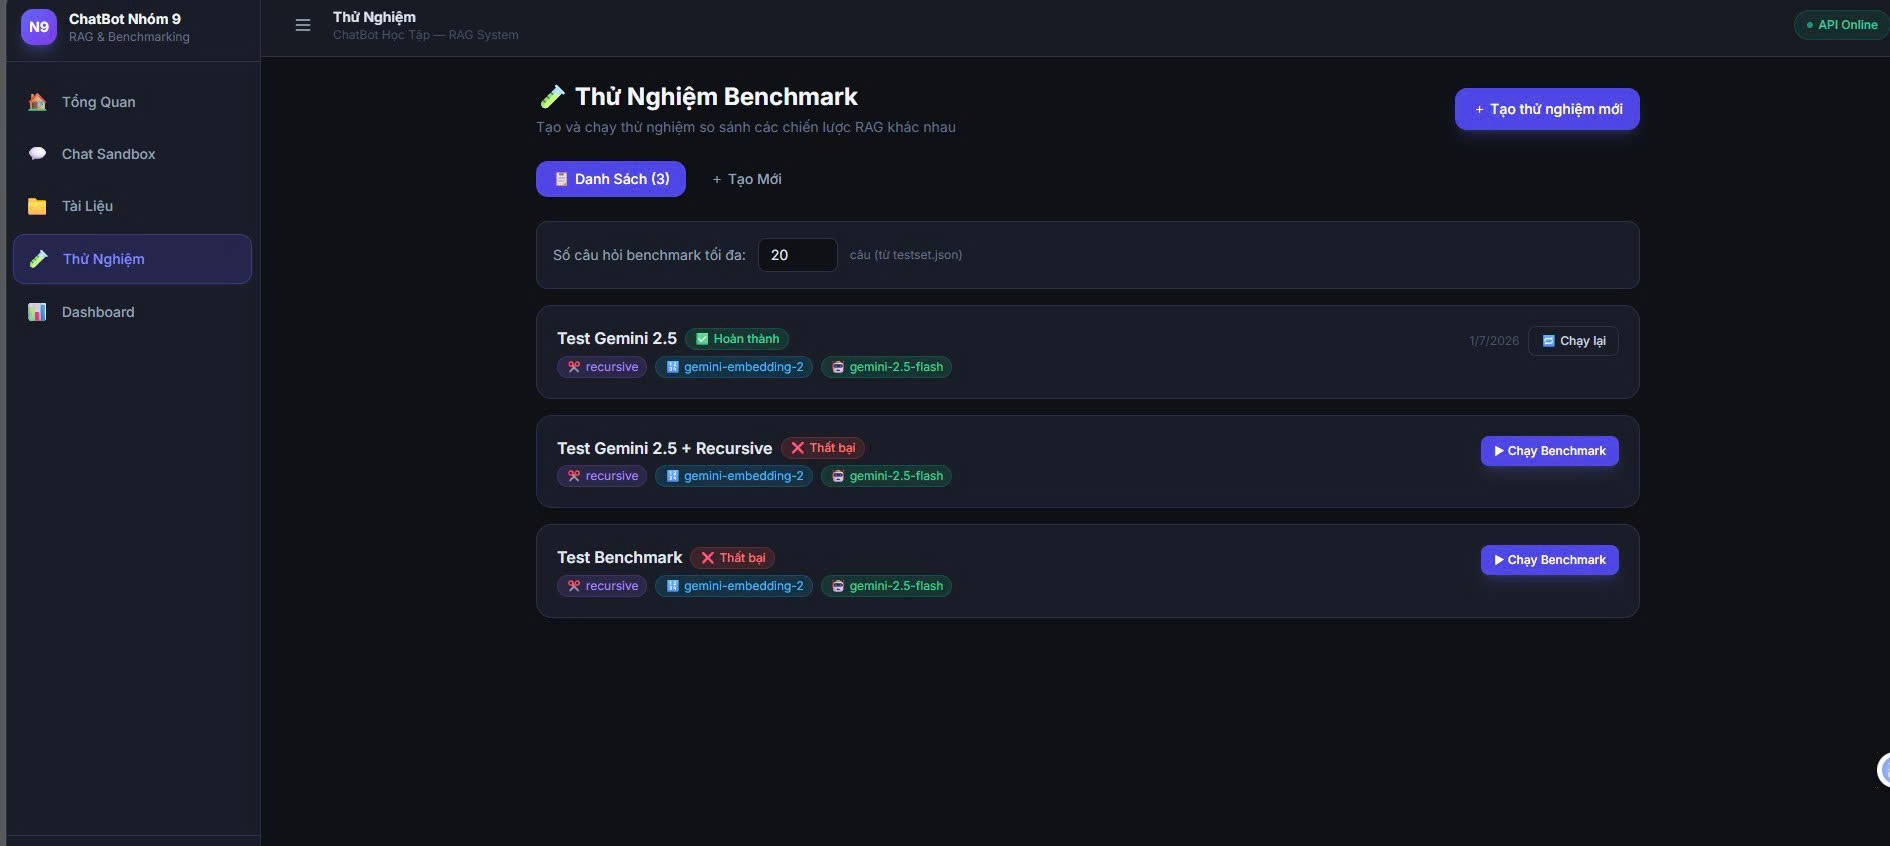
\includegraphics[width=\textwidth]{images/test_3}
	\caption{Chạy Benchmark}
	\label{fig:benchmark}
\end{figure}
Module Benchmark cho phép cấu hình:

\begin{itemize}
	\item Chunking Strategy
	\item Embedding Model
	\item AI Model
	\item Bộ câu hỏi kiểm thử
\end{itemize}

Sau khi chạy Benchmark, hệ thống tự động tính toán các chỉ số:

\begin{itemize}
	\item Accuracy
	\item Relevancy
	\item Faithfulness
	\item Latency
	\item Overall Score
\end{itemize}

Nhờ đó nhóm có thể đánh giá khách quan chất lượng của từng cấu hình RAG.
\section{Dashboard thống kê}

Sau khi hoàn thành Benchmark, toàn bộ kết quả được tổng hợp lên Dashboard.

\begin{figure}[H]
	\centering
	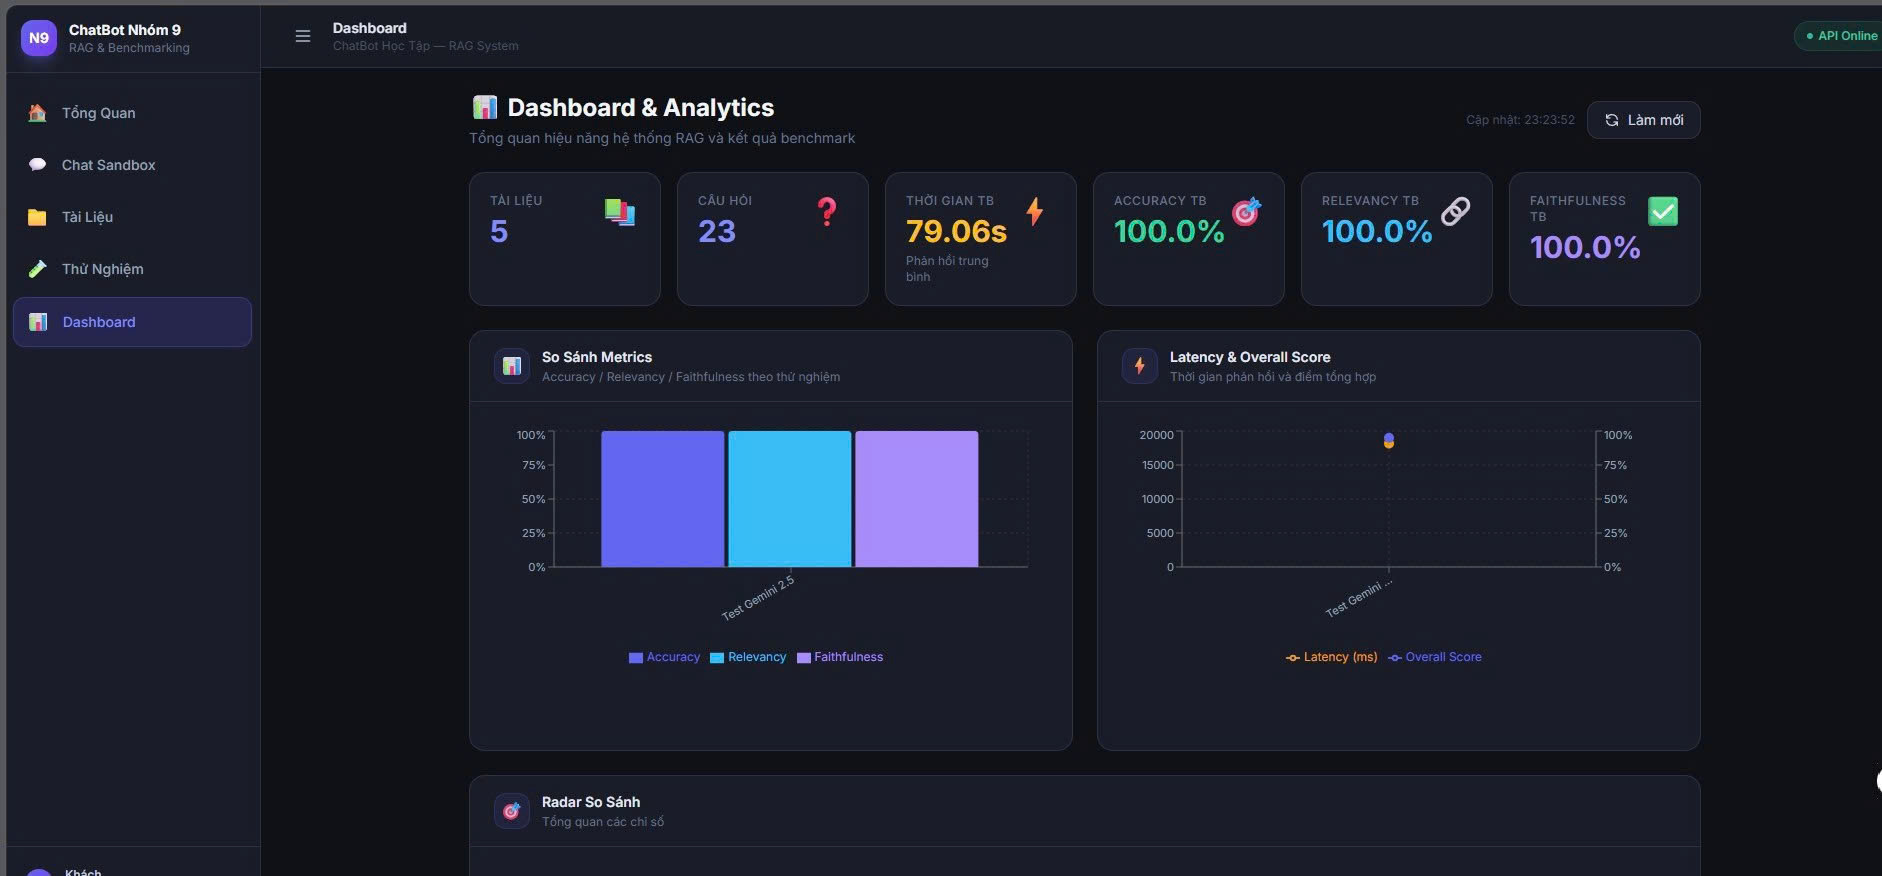
\includegraphics[width=\textwidth]{images/test_4}
	\caption{Dashboard tổng quan}
	\label{fig:dashboard}
\end{figure}
Dashboard hiển thị các chỉ số:

\begin{itemize}
	\item Số lượng tài liệu
	\item Số lượng câu hỏi
	\item Accuracy
	\item Relevancy
	\item Faithfulness
	\item Latency
\end{itemize}

Ngoài các chỉ số tổng quan, hệ thống còn hiển thị biểu đồ so sánh giúp người dùng dễ dàng quan sát sự khác biệt giữa các lần Benchmark.

\section{So sánh kết quả Benchmark}

\begin{figure}[H]
	\centering
	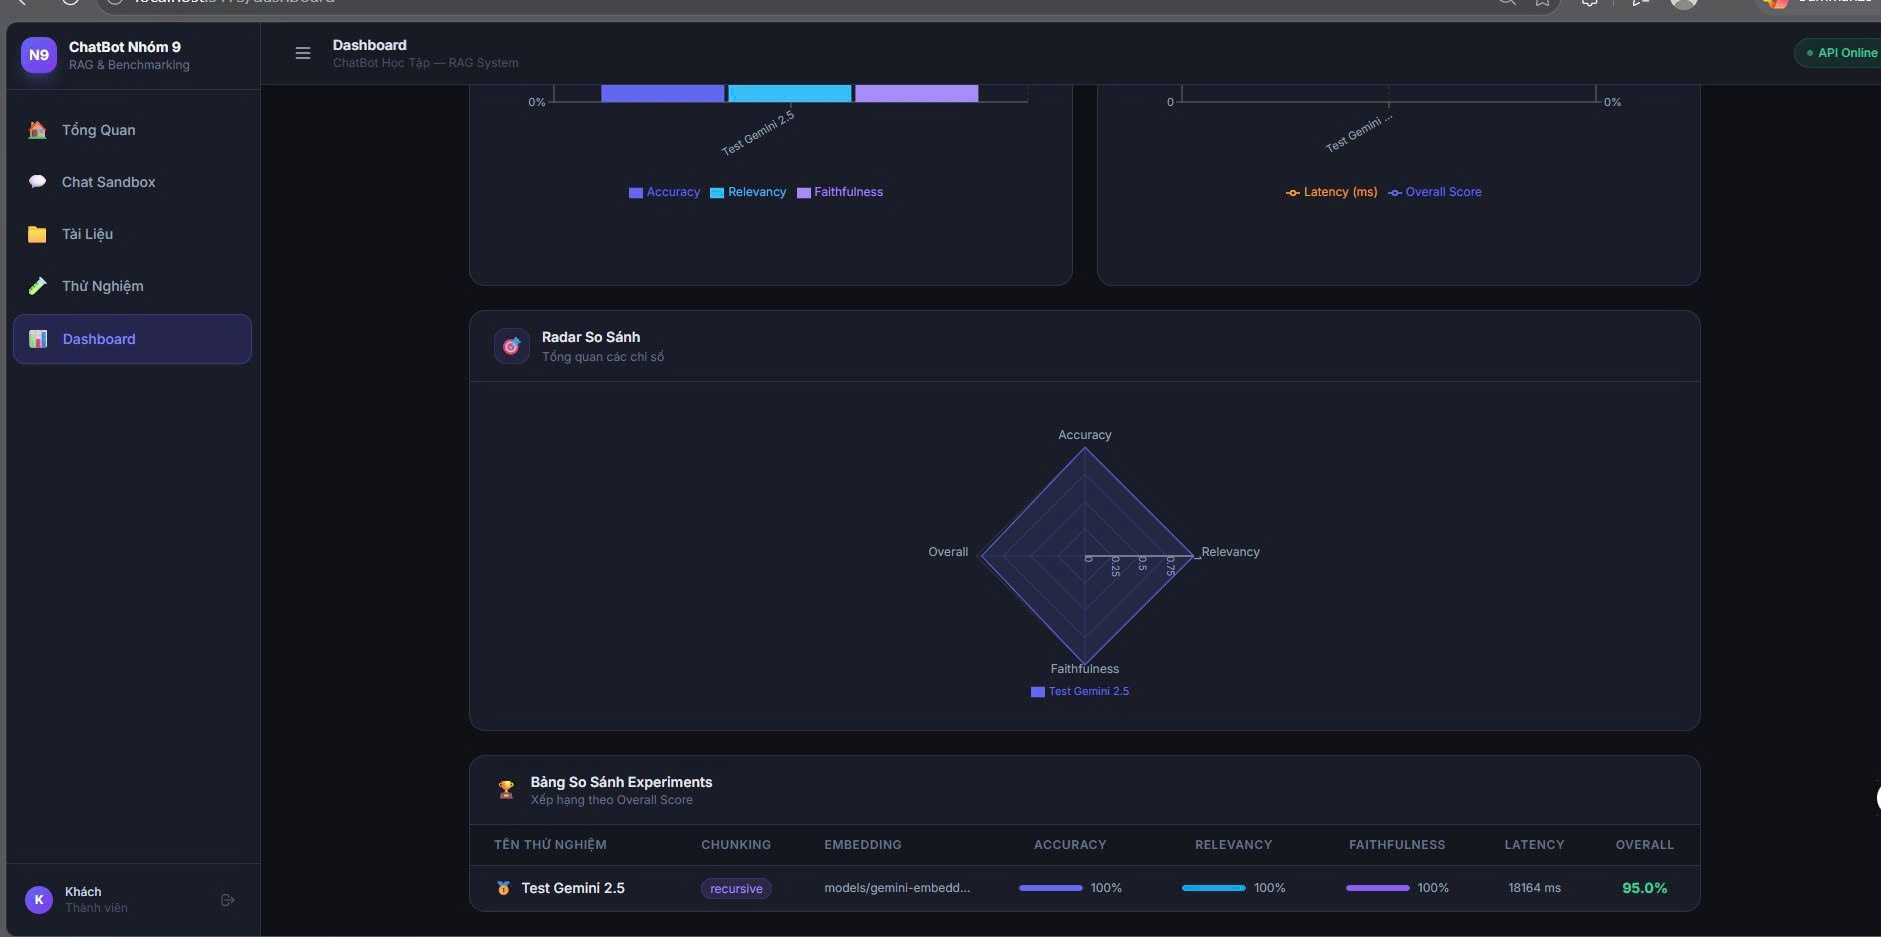
\includegraphics[width=\textwidth]{images/test_5}
	\caption{Biểu đồ Radar và bảng xếp hạng}
	\label{fig:radar}
\end{figure}
Radar Chart được sử dụng để trực quan hóa các chỉ số:

\begin{itemize}
	\item Accuracy
	\item Relevancy
	\item Faithfulness
	\item Overall Score
\end{itemize}

Bảng xếp hạng bên dưới hiển thị đầy đủ:

\begin{itemize}
	\item Tên thử nghiệm
	\item Chunking
	\item Embedding
	\item Accuracy
	\item Relevancy
	\item Faithfulness
	\item Latency
	\item Overall Score
\end{itemize}

Các chỉ số được tính toán tự động sau mỗi lần Benchmark và hỗ trợ nhóm lựa chọn cấu hình tối ưu.
\section{Đánh giá kết quả}

Sau quá trình kiểm thử, hệ thống đã đáp ứng đầy đủ các yêu cầu chức năng được đặc tả trong tài liệu SRS.

Các chức năng Upload tài liệu, Chat Sandbox, Benchmark và Dashboard đều hoạt động ổn định. Mô hình RAG kết hợp Gemini 2.5 Flash cho khả năng trả lời chính xác các câu hỏi thuộc phạm vi tài liệu được cung cấp.

Thông qua Dashboard và Benchmark, nhóm có thể đánh giá định lượng chất lượng của từng chiến lược Chunking và Embedding. Điều này giúp việc tối ưu hệ thống được thực hiện dựa trên dữ liệu thực tế thay vì cảm tính.

Kết quả kiểm thử cho thấy hệ thống đạt Accuracy, Relevancy và Faithfulness cao, đồng thời đảm bảo thời gian phản hồi phù hợp với yêu cầu của một chatbot hỗ trợ học tập.